\documentclass[preprint,11pt]{elsarticle}
\usepackage[T1]{fontenc}
\usepackage{lmodern,amsmath,amssymb,amsthm,booktabs,array,graphicx}
\usepackage{algorithm,algpseudocode}
\usepackage{pgfplots}
\pgfplotsset{compat=1.18}
\usepackage[hidelinks]{hyperref}
\usepackage[margin=1in]{geometry}
\usepackage{microtype}
\journal{Neurocomputing}
\makeatletter
\def\ps@pprintTitle{\let\@oddhead\@empty\let\@evenhead\@empty
\def\@oddfoot{\footnotesize Prepared for consideration in Neurocomputing\hfill\thepage}
\let\@evenfoot\@oddfoot}
\makeatother
\newtheorem{theorem}{Theorem}
\newtheorem{lemma}[theorem]{Lemma}
\newtheorem{proposition}[theorem]{Proposition}
\newtheorem{assumption}{Assumption}
\newcommand{\norm}[1]{\left\lVert#1\right\rVert}
\newcommand{\dist}{\operatorname{dist}}
\newcommand{\R}{\mathbb{R}}
\newcommand{\perm}{\mathfrak{S}}
\newcommand{\A}{\mathcal{A}}
\newcommand{\C}{\mathcal{C}}
\newcommand{\Live}{\mathcal{L}}
\newcommand{\eps}{\varepsilon}
\providecommand{\paperroot}{.}
\begin{document}
\begin{frontmatter}
\title{ChronoTrace: Conditional training-order verification by bidirectional replay}
\author{Omar Al-Tawil}
% Affiliation and corresponding email must be supplied and approved by the author.
\begin{abstract}
A final model checkpoint may be consistent with several orders of known training stages. Recovering one matching order does not exclude alternatives, while exhaustive replay can make verification expensive. We study this inverse problem for a known base and deterministic gradient-descent recipes. ChronoTrace joins forward prefix states with residual-controlled inverse-suffix enclosures, then replays surviving candidates against the checkpoint's rounding cell. Under global gradient regularity, invertible updates, and valid numerical allowances, the construction preserves every compatible history, including when inverse iterations or final replay are truncated. The contribution is a conditional endpoint-audit construction, not a new reversible-learning primitive. A source-locked study comprises 72 eight-stage digit-classification problems in 12 seed clusters, each observed through FP32 and FP16 checkpoint export; training and replay use FP64. All 72 FP32 observations yield unique verified candidates, versus nine correct first matches from a second-order ranked-replay baseline at matched gradient work. Median gradient work is 8.74 times lower than complete prefix-cached replay. Eight serial timing pairs give a 7.33-fold median speedup over that exhaustive reference. The strongest FP16 setting fails in all 24 cases despite unique exhaustive-reference solutions, exposing a limitation of uncertainty transport and the replay budget. A separate frozen-encoder, 170-parameter head experiment verifies 12 observations of six targets after more than 72\% head-loss reduction. The results support efficient auditing in a restricted known-recipe setting; they do not establish arbitrary-model provenance, subfactorial total computation, or formally validated floating-point certificates.
\end{abstract}
\begin{keyword}
Training chronology \sep Inverse learning dynamics \sep Model auditing \sep Set-membership inference \sep Reversible optimization \sep Checkpoint quantization
\end{keyword}
\end{frontmatter}

\section{Introduction}
Training pipelines often apply several adaptation stages to a common base. Even when the stage catalogue is known, an auditor may lack a reliable record of their order. The corresponding inverse question is narrower than identifying training data or establishing ownership: which permutations of the declared stages remain compatible with the final checkpoint? A useful answer may be a unique chronology, a partial order, or an explicit statement that the available evidence is insufficient.

Order-dependent learning and temporal information in trained models are not new phenomena. Reversible optimization has been used to differentiate through known training trajectories~\cite{maclaurin2015}. Temporal activation probes can recover acquisition-time information in language models~\cite{fresh2025}, while order correlations can support provenance testing when a randomized training transcript is known~\cite{palimpsest2025}. These results motivate endpoint auditing but do not remove the distinction between finding one matching history and excluding every alternative in a specified candidate model.

Exhaustive replay resolves this distinction directly: execute every possible history and compare its endpoint with the observation. Shared prefixes reduce redundant work, but the number of stage executions remains combinatorial. Approximate forward surrogates can rank candidates cheaply, yet a poor ranking or a loose approximation bound may respectively waste replay or prevent conservative exclusions. This paper investigates a different use of known training dynamics: compute candidate prefixes forward, undo candidate suffixes with explicit uncertainty, and reject incompatible combinations at their meeting point.

ChronoTrace is a set-valued auditor. It never interprets an unconverged inverse solve as evidence against a history, and it retains untested survivors when the replay cap is exhausted. Final verification uses the coordinate-wise rounding cell of the observed checkpoint, rather than treating export error as a freely tuned tolerance. The guarantee is conditional: the base, stage recipes, regularity bounds, and computation-error allowances must be valid, and the true process must belong to the declared candidate model. A unique output does not establish legal provenance or show that an unmodelled process could not produce the same endpoint.

The paper makes three scoped contributions. First, it formulates residual-controlled bidirectional joins for unknown-order endpoint auditing, with a no-loss result for compatible histories and a precise account of budget-induced abstention. Second, it supplies a reproducible evaluation that separates gradient work, actual runtime, first-match retrieval, and alternative exclusion. Third, it measures a failure boundary: stronger training combined with FP16 export makes the current inverse enclosures too broad, although the exhaustive candidate set remains uniquely identifiable. The proof ingredients---contraction mappings, inverse residual bounds, meet-in-the-middle enumeration, and set membership---are established tools; the claim concerns their particular audited composition and measured utility.

The main experiment concerns 64-dimensional logistic models, not large language models. An additional experiment audits only a 170-parameter head on a frozen learned encoder. These scales permit complete small-model references that would be impractical for larger pipelines. They provide controlled evidence about the mechanism and its cost, rather than a demonstration of production-ready reconstruction of arbitrary training histories.

\section{Related work}
\paragraph{Temporal information and provenance.}
\citet{fresh2025} show that training-order recency is linearly represented in language-model activations and study acquisition-time probes. This is a close inverse-temporal neighbour, so temporal traces themselves cannot establish novelty here. \citet{palimpsest2025} exploit correlations with a known randomized training order for black-box provenance testing. Proof-of-Learning instead uses records from training to support verification~\cite{jia2021}. ChronoTrace assumes neither a supplied order nor an intermediate checkpoint transcript, but requires substantially stronger access to a known base, gradients, and reproducible stage recipes. No empirical superiority over temporal probes or provenance systems is claimed; the present evaluation addresses a different, explicitly constrained output.

\paragraph{Forward order selection.}
Noncommuting gradient dynamics and Lie brackets explain order effects in multi-domain learning~\cite{rukhovich2025}. Geometric methods also predict favourable sequential training orders~\cite{sweeney2026}. These works principally concern choosing an order to improve learning. ChronoTrace infers an unknown order from an endpoint. This distinction does not make commutator reasoning new; indeed, the current decoder avoids relying on a global low-order commutator approximation for its main exclusion mechanism.

\paragraph{Reversibility and switching sequences.}
\citet{maclaurin2015} reverse known optimization trajectories for hyperparameter gradients. ChronoTrace uses approximate inversion of candidate suffixes, with residual bounds that remain valid before a numerical solver converges. Unknown sequence inference also appears in set-membership identification of switched systems. For example, \citet{ozay2015} infer subsystem models and switching sequences from noisy input--output data. Here the nonlinear stage maps are known and only their order is unknown; the observed training state is the endpoint rather than a full trajectory. Classical split enumeration~\cite{horowitz1974} supplies the computational pattern, not an additional novelty claim.

\paragraph{Position of the evidence.}
A same-information first-match baseline is essential because exhaustive candidate acquisition can make an elaborate inverse certificate unnecessary. We therefore compare against complete prefix-cached replay and second-order ranked replay, explicitly distinguishing their outputs. The earlier ChronoTrace secant certificate is retained as an internal ablation, not presented as an independent state-of-the-art comparator. Establishing performance against broader learned temporal decoders is outside this experiment and remains a limitation.

\section{Problem formulation and access assumptions}
Let $\theta_0\in\R^d$ be a known base state and let $\{1,\ldots,N\}$ index distinct training stages. Stage $i$ consists of $m_i$ gradient-descent updates,
\begin{equation}
 T_i(x)=x-\eta_i g_i(x),\qquad F_i=T_i^{m_i}.
\end{equation}
The experiments use fixed full-batch gradients within each stage. For an order $\pi\in\perm_N$, define
\begin{equation}
 x_\pi=F_{\pi_N}\circ\cdots\circ F_{\pi_1}(\theta_0).
\end{equation}
Each stage occurs exactly once. The observation is a finite exported checkpoint $y$, with a known coordinate-wise rounding cell $\C(y)$. A declared endpoint-computation allowance $\eps_y$ accounts for the discrepancy between exact dynamics and the numerically generated checkpoint before export. The compatible model class is
\begin{equation}\label{eq:compatible}
 \A(y)=\{\pi\in\perm_N:\dist(x_\pi,\C(y))\leq\eps_y\}.
\end{equation}
The auditor returns a superset $\Live(y)\supseteq\A(y)$. A precedence $a\prec b$ is reported only when it holds in every live order. If the model is assumed to contain the generating history and the live set is a singleton, that order is conditionally identified. An empty live set indicates inconsistency among the observation and assumptions, not which assumption failed.

\begin{assumption}\label{ass:regularity}
The base and recipes are fixed and known; each $g_i:\R^d\to\R^d$ is globally $L_i$-Lipschitz, and $q_i=\eta_i L_i<1$. Every used error allowance bounds the corresponding computation error in Euclidean norm.
\end{assumption}
The mathematical results apply to real-valued dynamics under Assumption~\ref{ass:regularity}. The reference implementation uses inflated numerical norm estimates and fixed guards, not outward-rounded interval arithmetic. Consequently, its numerical certificates are conditional on those allowances. The experiments audit deterministic plain GD; they do not justify applying the same routine to an unobserved momentum state, Adam, changing unknown minibatches, or an unknown base. A metadata signature catches ordinary recipe changes after prefix acquisition but does not authenticate hidden mutation within an arbitrary callback.

\subsection{Observation sets}
For an observed FP16 or FP32 coordinate $y_j$, let $y_j^-$ and $y_j^+$ be the adjacent representable values. A conservative closed rounding interval is
\begin{equation}\label{eq:cell}
 C_j=[(y_j^-+y_j)/2,\,(y_j+y_j^+)/2],\qquad
 \C(y)=\prod_{j=1}^d C_j.
\end{equation}
Both ties are included. Values whose neighbours overflow to infinity are rejected rather than assigned an unjustified finite interval. An FP64 observation is treated as a point with separate computation allowances. If $c$ is the box centre and $r_C$ its Euclidean half-diagonal, then $\C(y)\subseteq B(c,r_C)$. Inverse transport uses this enclosing ball; final replay uses the box itself. No hidden unrounded target is used to choose these intervals.

Training precision and observation precision are separate variables. All reported primary training, probing, inversion, and replay use FP64. FP32 and FP16 label only conversion of the observed final checkpoint. The results therefore cannot be interpreted as evidence for reconstruction of FP16-trained trajectories.


\section{Residual-controlled bidirectional verification}
\subsection{Inverse enclosure}
\begin{lemma}[Inverse residual bound]\label{lem:inverse}
Let $T(x)=x-\eta g(x)$, where $g$ is globally $L$-Lipschitz and $q=\eta L<1$. Then $T$ is bijective on $\R^d$, its inverse is $(1-q)^{-1}$-Lipschitz, and for approximate values $\widehat x,\widehat z$ and any $z$ with $\norm{z-\widehat z}\leq E$,
\begin{equation}\label{eq:inverse}
 \norm{\widehat x-T^{-1}(z)}
 \leq\frac{\norm{T(\widehat x)-\widehat z}+E}{1-q}.
\end{equation}
\end{lemma}
\begin{proof}
For each $z$, $x\mapsto z+\eta g(x)$ is a contraction on complete Euclidean space, so it has a unique fixed point satisfying $T(x)=z$. Also,
$\norm{T(x)-T(v)}\geq\norm{x-v}-\eta\norm{g(x)-g(v)}\geq(1-q)\norm{x-v}$.
Apply this inequality with $v=T^{-1}(z)$, then use the triangle inequality through $\widehat z$.
\end{proof}
A fixed-point solve proposes $\widehat x$. Its measured residual $r$ supplies the enclosure, not its convergence flag. With a justified residual-computation allowance $\delta$, propagate
\begin{equation}\label{eq:transport}
 E_{\rm previous}=\frac{E+r+\delta}{1-q}.
\end{equation}
The allowance must cover error in the residual evaluation and the proposed iterate as needed by the chosen implementation. Iteration exhaustion leaves this inequality valid when that allowance is valid; it increases $r$ rather than authorizing exclusion. In a suffix of $M$ reversed updates with common $q$, repeated application yields
\begin{equation}\label{eq:expansion}
 E_0\leq (1-q)^{-M}E_M+
 \sum_{j=1}^{M}(1-q)^{-j}(r_j+\delta_j),
\end{equation}
where the residuals are indexed in the corresponding reverse propagation order. This expression exposes both the benefit of small inverse residuals and the possible amplification of checkpoint uncertainty.

For forward computation, if an update is $G$-Lipschitz and the current radius is $e$, then $e'=Ge+\delta_f$. The general bound is $G\leq1+\eta L$. For the convex GD problems studied here, $G=1$ is justified by the stated step-size condition. Thus an order-independent bound for $Nm$ numerical updates is $\eps_y=Nm\delta_f$ in the common-step setting. Prefix states have their own accumulated computation radii; target computation is not silently assumed exact.

\subsection{The middle join}
Fix $1\leq k<N$. For every length-$k$ prefix $p$, compute its approximate endpoint $a_p$ with radius $e_p$. For every length-$(N-k)$ suffix $s$, reverse its updates from $c$ with initial radius $r_C+\eps_y$, obtaining an approximate inverse state $b_s$ and radius $E_s$. A prefix and suffix are considered together only if their stage sets are complementary.

\begin{theorem}[No-loss join and budget-safe refinement]\label{thm:no-loss}
Under Assumption~\ref{ass:regularity}, retain each complementary pair $(p,s)$ satisfying
\begin{equation}\label{eq:join}
 \norm{a_p-b_s}\leq e_p+E_s.
\end{equation}
Then every order in $\A(y)$ survives the join. If a joined order is replayed to $\widehat x_\pi$ with endpoint error bound $e_\pi$, it can be excluded when
\begin{equation}\label{eq:exclude}
 \dist(\widehat x_\pi,\C(y))>e_\pi+\eps_y.
\end{equation}
Retaining all untested joined orders at any replay stopping point gives a live set containing $\A(y)$.
\end{theorem}
\begin{proof}
Every permutation has a unique split $\pi=p+s$ with complementary stage sets. If $\pi\in\A(y)$, its endpoint lies in $B(c,r_C+\eps_y)$. Inverse transport therefore encloses its exact middle state $z$. Forward propagation encloses the same state, so $\norm{a_p-b_s}\leq\norm{a_p-z}+\norm{z-b_s}\leq e_p+E_s$. For refinement, distance to any nonempty closed set is 1-Lipschitz. Thus
$\dist(\widehat x_\pi,\C(y))\leq\norm{\widehat x_\pi-x_\pi}+\dist(x_\pi,\C(y))\leq e_\pi+\eps_y$ for every compatible order. Neither allowed exclusion removes a member of $\A(y)$; leaving untested orders unchanged preserves this invariant.
\end{proof}
Implementation guards enlarge the right-hand sides of the tests. Their adequacy is a numerical assumption, not a consequence of the real-arithmetic theorem. The theorem permits unfinished inverse iterations because the residual enclosure remains available, but it requires the prefix and suffix catalogues to be complete. A truncated catalogue would need an explicit representation of all unexplored histories and is not the implemented algorithm.

\begin{proposition}[Conditional order inference]
If $\A(y)$ is nonempty and $\Live(y)$ has one element, its element is the unique compatible order. Any precedence shared by all live orders holds for every compatible order.
\end{proposition}
\begin{proof}
Both statements follow from $\varnothing\ne\A(y)\subseteq\Live(y)$.
\end{proof}
The implementation labels a singleton that passes replay and has no untested alternatives \texttt{verified\_unique}. This denotes numerical replay consistency plus conditional alternative exclusion. The replay tolerance is a necessary enclosure test, not an unconditional existence proof that an exact endpoint lies inside the unexpanded rounding cell. The nonempty candidate-model assumption remains essential.

\subsection{Algorithm and accounting}
Algorithm~\ref{alg:chrono} states the decision procedure. Candidate generation and decisions do not receive the generating order. Batched evaluations are charged once per evaluated parameter vector, including every inverse residual check. The replay cap covers suffix replay; it is not a cap on total prefix and inverse acquisition.

\begin{algorithm}[t]
\caption{Conditional bidirectional chronology audit}\label{alg:chrono}
\begin{algorithmic}[1]
\Require Base, $N$ stage recipes, split $k$, observation cell, valid allowances, replay cap
\State Acquire all length-$k$ forward prefixes with error radii; cache shared prefixes
\State Acquire all reverse suffixes of length $N-k$ using residual-controlled inverse updates
\State $J\gets$ all complementary prefix--suffix pairs satisfying the middle test
\State $\Live\gets J$
\For{candidate $\pi\in J$ in a fixed label-independent order}
  \If{the next suffix replay exceeds the remaining replay cap}
    \State \textbf{break} \Comment{Untested candidates remain live}
  \EndIf
  \State Replay its suffix from the cached prefix and propagate forward error
  \If{the endpoint is excluded by Eq.~\eqref{eq:exclude}}
    \State Remove $\pi$ from $\Live$
  \EndIf
\EndFor
\State Return $\Live$, its common precedences, and the accounting/abstention status
\end{algorithmic}
\end{algorithm}

Write $P(N,r)=N!/(N-r)!$ and $A(N,k)=\sum_{r=1}^k P(N,r)$. With $m$ updates per stage, prefix acquisition costs $mA(N,k)$ gradients. Inverse acquisition has $A(N,N-k)$ stage calls, but its gradient count depends on measured residual iterations and is reported directly. The split is selected without the target by minimizing $A(N,k)+cA(N,N-k)$ for a declared inverse/forward cost estimate $c$. With $N=8,c=8$, it selects $k=5$: 8,800 forward-prefix and 400 inverse-suffix stage calls. Complete shared-prefix replay costs $mA(8,8)=32\times109,600=3,507,200$ gradients.

This is not a subfactorial total-computation result. The reference implementation compares all $N!$ complementary middle pairs. It stores combinatorial catalogues, and weak exclusions can leave factorially many candidates for verification. Prefix construction can be amortized across targets sharing recipes, but the reported comparison charges the cold prefix cost to every observation; target generation and exhaustive reference construction are charged separately to the evaluator.


\section{Experimental design}
\subsection{Evidence roles and independence}
The primary method, tolerances, task grid, seeds, and source hashes were locally locked before fresh-seed execution. This was not external preregistration. All locked cells are retained, including the anticipated strong-training/FP16 stress cell. Historical Pythia terminal and nonterminal-secant studies informed method development; they are not pooled into the primary sample or relabelled as fresh evidence.

The design uses 12 seeds, two task families, three stage durations, and two export formats. There are 72 problem-specific endpoints and 144 observations. The target permutation is a deterministic function of the seed alone, so only \emph{12 distinct sampled orders} occur; each is reused across six task/duration problems and both exports. Random stage partitions and target permutations share this seed-cluster structure. The dataset is also shared. Accordingly, the observations are not 144 independent histories, and the 4,032 possible pair decisions are not independent statistical trials.

\subsection{Binary digit-classification problems}
We use the 1,797-example, 64-feature \texttt{load\_digits} subset distributed with scikit-learn, derived from the Optical Recognition of Handwritten Digits dataset~\cite{digits1998,sklearndigits}. Pixel values are divided by 16, then each feature row is divided by the larger of one and its Euclidean norm. A seed-dependent permutation assigns 80\% of examples (1,437) to adaptation and the remaining 360 to evaluation. Adaptation examples are split into eight nearly equal, disjoint stage blocks. These are random data blocks of the same task, not eight independently collected semantic domains.

The two targets are parity and whether the digit is at least five. For stage matrix $X_i$ and binary labels $t_i$, the objective is logistic cross-entropy with ridge coefficient $\lambda=10^{-3}$. The gradient is
\begin{equation}
 g_i(w)=X_i^\top(\sigma(X_iw)-t_i)/n_i+\lambda w,
\end{equation}
with $L_i\leq\norm{X_i}_2^2/(4n_i)+\lambda$. The implementation computes the spectral norm numerically and multiplies the bound by $1+10^{-12}$. Each stage has $m=32$ updates, step size $\eta=\tau/m$, and duration $\tau\in\{5,10,20\}$. All configured steps satisfy $\eta L_i<1$. This use of analytic curvature structure is an access advantage relative to methods requiring only executable stage maps.

The numerical protocol uses a per-update allowance of $10^{-12}$, join allowance $10^{-10}$, inverse residual tolerance $10^{-12}$, at most 24 inverse iterations per update, and at most 300,000 replay gradients. Rounding cells are computed from exported observations alone. The software stack is NumPy 2.3.5, SciPy 1.17.0, and scikit-learn 1.8.0; full source and dataset hashes are included in Supplement S1. Held-out task accuracy is a descriptive check that learning is nontrivial, not the criterion used to select the auditor. Random image-level splitting does not establish writer-disjoint generalization.

\subsection{References and comparators}
\paragraph{Complete prefix-cached replay.}
An evaluator enumerates all 40,320 endpoints for each of the 72 problems after decoder predictions are fixed. Its compatible set uses the same observation box and declared computation allowances. This permits checking whether any reference-compatible alternative was lost, not only whether the generating order was guessed. Stored raw arrays retain all order indices, endpoint-to-cell distances, observation boxes, and decoder live sets; endpoint tensors themselves are recomputable rather than all retained. This is an independent computational path in the same environment, not an external replication or a formal numerical oracle.

\paragraph{Second-order ranked replay.}
Singleton and ordered-pair probes define a second-order endpoint surrogate. The comparator ranks all permutations by their surrogate distance to the observed cell centre, then replays candidates until the first compatible endpoint or its work cap. Shared prefixes and the initial probes are charged. Its budget equals the new method's realized total gradient count, including cold prefix acquisition. Ranking does not read the generating label. The exhaustive reference is used only to score the exact cached-prefix work at which the ranked sequence would first reach a compatible candidate. Consequently, this is a work-budget comparison, not a timed standalone implementation of ranked replay. A first match is also a weaker output than alternative exclusion.

\paragraph{Earlier secant certificate.}
The preceding ChronoTrace method uses low-order probes, a finite-stage remainder bound, adaptive candidate refinement, and selective replay. It receives an enclosing ball for the same checkpoint cell, a 20,000-node search cap, and a comparable stage-work allowance for refinement. This internal ablation tests whether the previous global forward approximation remains useful at the stronger settings; it is not a literature-wide benchmark.

\subsection{Timing and learned-representation bridge}
A separately locked serial timing study repeats eight spent FP32 inputs: the first two primary seeds, both families, and durations 5 and 20. Each method is executed once per input, on one CPU thread, with order alternated. Both timings include cold candidate acquisition and decoding, but exclude task preparation and target generation. No standalone ranked-replay runtime is claimed. The original timing artifact does not record the CPU model, limiting hardware reproducibility; per-input times and thread settings are retained.

A separate bridge trains a 64-to-16 tanh encoder on a disjoint 40\% data split and freezes it. Another 40\% supplies the eight audited head stages; the final 20\% is held out. Tanh features plus a bias coordinate form a 17-dimensional input, normalized to row norm at most one. Only a $17\times10$ softmax head is audited. Its ridge coefficient is $10^{-3}$ and a valid global gradient bound is $\norm{X_i}_2^2/(2n_i)+\lambda$. Six new target seeds, $m=32$, and $\tau=10$ give 12 FP32/FP16 observations. The targets share the encoder and dataset. Only the first predeclared seed is fully enumerated; the other five are not independently exhaustively checked. A stronger duration-20/FP16 development failure is retained separately, not promoted into confirmation.

\subsection{AI-assisted development and analysis}
ChatGPT (OpenAI) was used interactively for algorithm development, proof drafting and checking, code generation, test design, experiment orchestration, analysis, and literature discovery. The implementation and source locks record the executable decisions; reported numerical outcomes come from those computations, not language-model predictions. AI-generated proposals were exercised by unit tests, residual checks, and the separately executed endpoint references described above. These checks do not constitute independent human peer review. The research artifacts do not preserve a versioned model-build identifier for every AI-assisted interaction. The result figure is a deterministic PGFPlots rendering of the six aggregate counts in Table~\ref{tab:coverage}; its source is supplied, and no synthetic experimental data or generated primary research image is used.


\section{Results}
\subsection{Coverage, abstention, and alternative retention}
Table~\ref{tab:coverage} reports every primary cell. ChronoTrace verifies all 72 FP32 observations, whereas ranked replay reaches nine matching histories at the same gradient-work budgets. At FP16, all 48 observations with durations 5 and 10 are verified, but no observation at duration 20 is verified. Ranked replay instead succeeds in eight of those 24 strong-FP16 cases. Thus the new method does not dominate ranked retrieval across the entire grid.

\begin{table}[t]
\centering
\caption{Primary results. Each row has 24 observations (12 seed clusters and two task families). ``Verified'' includes conditional uniqueness and numerical replay consistency; ``retrieved'' is a first match. Both exports observe the same 72 endpoints.}\label{tab:coverage}
\begin{tabular}{llrrr}
\toprule
Export & Duration & ChronoTrace verified & Ranked retrieved & Secant verified\\
\midrule
FP32 & 5 & 24/24 & 3/24 & 0/24\\
FP32 & 10 & 24/24 & 3/24 & 0/24\\
FP32 & 20 & 24/24 & 3/24 & 0/24\\
FP16 & 5 & 24/24 & 3/24 & 0/24\\
FP16 & 10 & 24/24 & 3/24 & 0/24\\
FP16 & 20 & 0/24 & 8/24 & 0/24\\
\midrule
Total & & 120/144 & 23/144 & 0/144\\
\bottomrule
\end{tabular}
\end{table}
Across all primary observations, 3,360 of 4,032 possible unordered-pair relations are inferred, with no observed wrong pair or full-order output. All reference-compatible orders are retained. The exhaustive compatible set is a singleton for every problem/export pair, including every strong-FP16 failure. The latter failures therefore demonstrate limited pruning under the implemented uncertainty bounds and replay cap, not established information-theoretic non-identifiability.

At duration 20 with FP16 export, all 40,320 middle candidates survive in these runs; the replay cap permits 3,125 suffixes and leaves 37,195 untested candidates. No common pairwise relation is then reported. Their unique exhaustive solutions remain present. Across the primary study, mean training-loss reduction ranges from 9.03\% to 39.53\%, and held-out classification accuracy ranges from 73.33\% to 87.78\%. These measures exclude the interpretation that the primary successes concern only infinitesimal parameter updates.

For FP32, the paired coverage difference relative to ranked first-match retrieval is 87.5 percentage points. A descriptive bootstrap resamples the 12 seed clusters with replacement, preserving all conditions within each selected cluster; 20,000 replicates with seed 55167 give a percentile interval of 76.4--97.2 points. This interval describes variation among the sampled seed clusters on a fixed dataset. It is not a guarantee over independent datasets or realistic pipelines. Zero observed mistakes likewise does not establish a population error rate of zero.

\subsection{Gradient work and runtime}
Table~\ref{tab:work} separates work from success. FP32 total work is a median of approximately $4.01\times10^5$ gradients, versus 3,507,200 for complete prefix-cached replay. The median exhaustive/new ratio is 8.74, ranging from 8.21 to 9.14. No endpoint-reference acquisition is hidden in the new decoder's budget. FP16 work increases when uncertainty leaves more candidate replays; this additional spending still fails to verify the strongest cell.

\begin{table}[t]
\centering
\caption{Median total gradient evaluations and maximum inverse radius within each observation, aggregated by cell. Prefix, inverse, residual-check, and verification work are included. The exhaustive reference uses 3,507,200 gradients in every cell.}\label{tab:work}
\begin{tabular}{llrr}
\toprule
Export & Duration & Median gradients & Median inverse radius\\
\midrule
FP32 & 5 & 384,015.5 & $1.36\times10^{-6}$\\
FP32 & 10 & 401,366.0 & $3.38\times10^{-5}$\\
FP32 & 20 & 415,942.0 & $1.67\times10^{-2}$\\
FP16 & 5 & 384,706.5 & $1.11\times10^{-2}$\\
FP16 & 10 & 447,889.0 & $2.76\times10^{-1}$\\
FP16 & 20 & 714,252.5 & $1.36\times10^{2}$\\
\bottomrule
\end{tabular}
\end{table}

The eight serial timing pairs yield a median ChronoTrace time of 1.824 seconds and a median exhaustive time of 13.214 seconds. The median of the paired ratios is 7.33, with a range of 6.70--15.46. The largest ratio includes a 25.93-second exhaustive run; retaining this outlier avoids selective reporting, and the paired median reduces its influence. All repeated outputs agree with the exhaustive reference. These are same-environment repeat checks on spent inputs, not new independent confirmation. Timings do not establish an asymptotic speedup, and machine-specific performance should be remeasured with recorded hardware.

\begin{figure}[t]
\centering
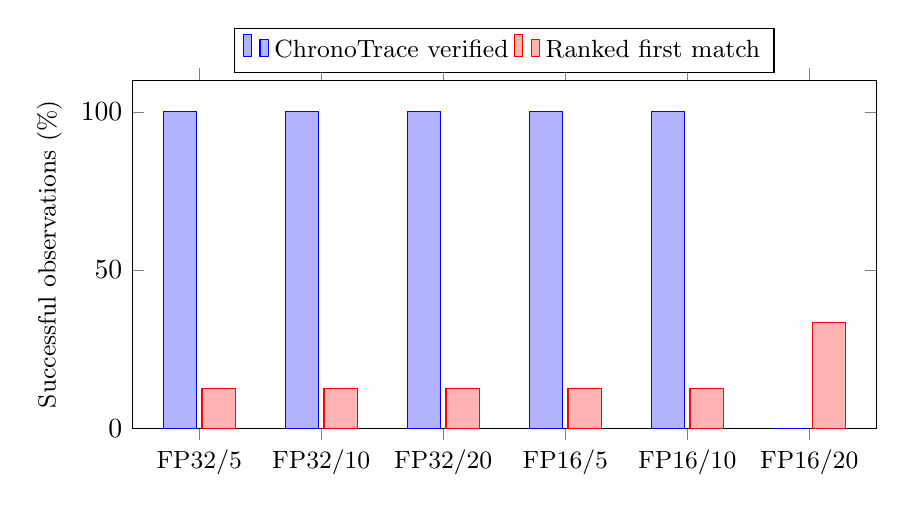
\begin{tikzpicture}
\begin{axis}[width=.91\linewidth,height=6.0cm,ybar,bar width=12pt,
 ymin=0,ymax=110,ylabel={Successful observations (\%)},
 symbolic x coords={32/5,32/10,32/20,16/5,16/10,16/20},xtick=data,
 xticklabels={FP32/5,FP32/10,FP32/20,FP16/5,FP16/10,FP16/20},
 x tick label style={font=\small},ylabel style={font=\small},
 legend style={at={(.5,1.02)},anchor=south,legend columns=2,font=\small},
 enlarge x limits=.11]
\addplot coordinates {(32/5,100)(32/10,100)(32/20,100)(16/5,100)(16/10,100)(16/20,0)};
\addplot coordinates {(32/5,12.5)(32/10,12.5)(32/20,12.5)(16/5,12.5)(16/10,12.5)(16/20,33.3333)};
\legend{ChronoTrace verified,Ranked first match}
\end{axis}
\end{tikzpicture}
\caption{Coverage by export format and stage duration at matched gradient-work budgets (24 observations per cell). Verification and first-match retrieval are different outputs. The strong-FP16 reversal is retained. Training and replay remain FP64 throughout.}
\label{fig:coverage}
\end{figure}


\subsection{Learned frozen encoder}
All 12 checkpoint observations in the head-only bridge yield uniquely verified candidates, with no observed wrong pair or full order. Head-loss reduction is 72.31--72.46\%, while held-out accuracy is 95.83--96.94\%. Both export formats for the one completely enumerated target agree with the reference. The other five targets have conditional decoder outputs and generating-label checks, but no exhaustive alternative-set cross-check.

This bridge supports a limited generalization: the audit can survive a large measured learning change in a head attached to a nonlinear learned representation. It does not establish recovery of the encoder's training trajectory, joint deep-network dynamics, or language-model adaptation. The encoder reaches its declared 200-epoch limit; no optimization-convergence result is claimed.


\section{Discussion and limitations}
\paragraph{What is measurably useful.}
For a known-recipe audit, complete enumeration supplies an expensive reference answer. The measured work and runtime reductions show that explicitly joining forward and inverse information can reach the same unique answer more cheaply in a controlled, nontrivial learning regime. The improvement concerns training-stage computation under these conditions. It is not evidence of general commercial return, production robustness, or a new lower bound on sequence-search complexity.

\paragraph{Why the precision boundary matters.}
Equation~\eqref{eq:expansion} makes checkpoint uncertainty and training contraction interact. Reversing a more contractive sequence amplifies observation uncertainty. The FP16 failures retain tens of thousands of alternatives even though only one candidate is compatible with the exact numerical reference. Tighter set transport, anisotropic enclosures, or adaptive splitting could improve this boundary, but such extensions have not been evaluated here. Nor does success at FP32 imply that a real FP32-trained pipeline can be inverted with the same recipe.

\paragraph{Assumption validity and model mismatch.}
Known executable maps are not enough for the guarantee: correct global regularity and numerical bounds are also required. A declaration of nonexpansiveness must be justified by the dynamics, not inferred from a few observed contractions. Unknown minibatches, persistent optimizer state, repeated or missing stages, an unknown base, and export transformations beyond the specified formats fall outside the confirmed model. Tests reject several malformed and inconsistent inputs, but the experiments do not calibrate false acceptance for realistic out-of-model processes. Even a unique in-model explanation is not proof that the true process was in model.

\paragraph{Numerical and statistical confidence.}
The exact-arithmetic invariant is proved, and exhaustive small references exercise the implemented decisions. Fixed numerical guards and numerically estimated spectral norms are nevertheless not formal floating-point verification. Source hashes establish artifact identity, not mathematical truth. Reproduction in one environment does not replace specialist proof review or external replication. The shared dataset, twelve sampled primary orders, and head-only bridge limit statistical generalization. A much wider task suite, larger components, and calibrated temporal baselines would be needed for a broad forensic claim.

\paragraph{Cost and comparison boundaries.}
Complete middle matching remains factorial, and the current storage pattern is combinatorial. The timing study does not benchmark standalone ranked replay. Ranked retrieval wins in the strong-FP16 cell and can be preferable when finding one plausible explanation is sufficient. ChronoTrace is useful when conditional exclusion of alternatives is required and known dynamics permit tight enough inverse transport. Applications should choose the weaker or stronger output deliberately rather than conflate them.

\section{Conclusion}
ChronoTrace combines forward prefixes, residual-controlled inverse suffixes, and checkpoint rounding cells to perform conditional training-order verification without first replaying every complete history. Its no-loss invariant makes nonconvergence and replay-budget exhaustion explicit sources of uncertainty rather than hidden exclusions. In the reported eight-stage reference problems, all FP32 observations are uniquely verified with a median 8.74-fold reduction in gradient work; a small serial study measures a 7.33-fold median speedup over exhaustive replay. The strong-FP16 failure and the limited frozen-encoder bridge delimit that result. The supported contribution is a reproducible, assumption-explicit audit method with measured computational value, not unrestricted model provenance or universally efficient history recovery.

\section*{Data and code availability}
The native implementation, tests, theory note, and manuscript source are maintained in \url{https://github.com/Null-Square/chronotrace}. The publication preparation is tracked in pull request 16. The frozen engine commit is recorded in Supplement S1 and the repository evidence ledger. Supplement S1 is the accompanying complete research archive, containing the locally locked protocols, experimental drivers, dependency pins, raw candidate-distance arrays, live sets, and artifact verifier. The supplementary README specifies exact hashes and reproduction commands. The source dataset is public and separately attributed~\cite{digits1998,sklearndigits}.

\appendix
\section{Implementation and reproducibility details}
The frozen primary protocol SHA-256 is
\begin{quote}\small\ttfamily
931b5e2caa42a9d707ade143b9da9a22360ee0f10e9255dfe21a9c508ac1a0e5.
\end{quote}
The record-file SHA-256 is
\begin{quote}\small\ttfamily
0da6ba2e6b06e65d1d640bfa79ea8cce187a2079cce3dbc9bbd26e336efb5181.
\end{quote}
The 12 primary seeds are 352021688, 399760960, 500317727, 570978561, 615840300, 925333088, 953947831, 1560033684, 1681784917, 1832827134, 1906214354, and 2003918457. The target-order generator uses \texttt{default\_rng(seed XOR 0x52ac9481)}. A source-lock check precedes execution, and the runner refuses dataset or declared dependency-version drift. Original output directories are not reused for reruns.

The 124 bidirectional test items include all 24 four-stage orders on 12 affine problems at three precisions (864 order-level comparisons), exhausted inverse iterations, genuine ambiguity, replay caps, rounding cells, mutation isolation, invalid inputs, and accounting. The accompanying standalone workspace passes 1,073 test items, including earlier secant and closure tests. These counts describe different test collections from the native repository regression suite. An additional publication-branch CI run executes the full native repository tests in normal and optimized Python; this is software validation, not new scientific sample size.

A compact independent audit extracts Supplement S1, installs the pinned requirements, and runs:
\begin{verbatim}
export OPENBLAS_NUM_THREADS=1 OMP_NUM_THREADS=1
export PYTHONPATH=src:scripts
python scripts/verify_bidirectional_artifacts.py --root .
python -m pytest -q tests
python -O -m pytest -q tests
\end{verbatim}
The verifier checks seven primary source hashes, the complete 144-case grid, 72 raw problem files, candidate-set retention, work identities, and reported decisions. It recomputes conclusions from stored distances; it does not independently regenerate those distances. The full training/reference runner is required for computational replication:
\begin{verbatim}
python scripts/run_bidirectional_confirmation.py \
  --config configs/bidirectional_v1.lock.json \
  --output artifacts/independent_rerun --workers 1
\end{verbatim}
The evaluator's exhaustive computation is intentionally outside the decoder's budget, and its output must not be fed back into decisions. Hardware, operating system, BLAS implementation, and CPU affinity should be recorded for any new runtime study.

\section{Neural-bridge protocol}
A fixed split generator with seed 2026091257 partitions the 1,797 examples into 718 encoder-training, 719 head-adaptation, and 360 held-out examples. The encoder is a scikit-learn multilayer perceptron with 16 tanh hidden units, Adam learning rate 0.01, regularization 0.001, batch size 64, 200-epoch limit, seed 71907, tolerance $10^{-6}$, no early stopping, and patience 200. Features are frozen before the six fresh head-seed runs. The audited softmax head starts from zero and uses 32 updates per stage at duration 10. The protocol and raw files disclose the complete six-seed list and separately retained pilot failures. Its primary scientific claim is head-only recovery; encoder-training randomness is not independently replicated across the six targets.

\section{Historical evidence boundary}
Earlier repository results concern different methods and access regimes. A four-stage Pythia-14M terminal witness experiment reports 27/32 full histories; later logical closure yields 28/32 post hoc, while stored discrete endpoint statistics resolve 32/32. These terminal comparisons already acquire complete candidate endpoints and therefore do not establish the current bidirectional efficiency claim. A subsequent 1,440-case nonterminal secant study uses small reference problems and is likewise not pooled with the primary bidirectional confirmation. Original protocol locks and outcomes remain unchanged. The current article is based on the bidirectional study and its supplementary evidence rather than the superseded manuscript narrative.

\section*{Declaration of generative AI and AI-assisted technologies in manuscript preparation}
ChatGPT (OpenAI) supported manuscript organization, drafting, literature discovery, reference organization, mathematical exposition, and preparation of reproducible data-visualization code. Its role in the research process is described in the Methods. AI assistance does not constitute independent peer review or external replication, and no AI system is credited as an author. The human author remains responsible for the accuracy, interpretation, originality, and final approval of the submitted work.



\bibliographystyle{elsarticle-num-names}
\bibliography{\paperroot/references}
\end{document}
